\chapter{Ayrılma Aksiyomları}
\label{ch:separation}

%% ============================================================
\section{Konu}
%% ============================================================

Ayrılma aksiyomları, bir topolojik uzaydaki noktaların ve kapalı kümelerin birbirinden
açık kümeler aracılığıyla ne ölçüde ``ayrılabildiğini'' ölçer.

\begin{sezgi}
Ayrılma aksiyomlarını bir mikroskobun çözünürlük kademeleri gibi
düşünün: T0'da iki noktayı \emph{en az bir yönden} ayırt edebilirsiniz;
T1'de her iki yönden; T2'de noktaları çakışmayan iki ayrı ``görüş
alanına'' koyabilirsiniz; T3 ve T4'te artık nokta--kapalı küme ve
kapalı--kapalı çiftleri bile ayrışır. Matematiksel karşılığı: her
aksiyom, $\tau$'nun ``ayırma gücü'' üzerine gittikçe güçlenen bir
varsayımdır ve zincir boyunca her adım bir öncekini gerektirir.
\end{sezgi}

\begin{table}[h]
\centering
\begin{tabular}{lll}
\toprule
\textbf{Aksiyom} & \textbf{İsim} & \textbf{Koşul} \\
\midrule
T0 & Kolmogorov & $\forall x \neq y$: $\exists U \in \tau$ ayıran \\
T1 & Fréchet & $\forall x \neq y$: iki yönlü ayrım \\
T2 & Hausdorff & $\forall x \neq y$: disjoint $U \ni x$, $V \ni y$ \\
T2.5 & Urysohn & disjoint kapanışlı komşuluklar \\
T3 & Regüler & T1 + nokta/kapalı ayırma \\
T3.5 & Tychonoff & T1 + sürekli fonksiyon ayırma \\
T4 & Normal & T1 + disjoint kapalılar ayırma \\
\bottomrule
\end{tabular}
\caption{Ayrılma aksiyomları}
\end{table}

\noindent\textbf{Sıralama:} T4 $\Rightarrow$ T3.5 $\Rightarrow$ T3 $\Rightarrow$ T2.5
$\Rightarrow$ T2 $\Rightarrow$ T1 $\Rightarrow$ T0.

\begin{dikkat}
T3 ve T4'ün tanımı kaynaktan kaynağa değişir: bazı kitaplar
``regüler''i T1 olmadan tanımlar. Bu kılavuzda ve \texttt{pytop}'ta
tablodaki konvansiyon geçerlidir: \textbf{T3 = T1 + regüler,
T4 = T1 + normal}. Fark gerçektir: iki noktalı indirgenmiş uzay
regüler \emph{ve} normaldir (ayrılacak uygun çift yoktur), ama T1
olmadığından T3 de T4 de değildir; Örnekler bölümünde
\texttt{is\_regular}/\texttt{is\_t3} ile doğrulanır.
\end{dikkat}

Şekil~\ref{fig:ch06:t2} Hausdorff koşulunu, Şekil~\ref{fig:ch06:t3}
regülerlik koşulunu resmeder.

\begin{figure}[ht]
  \centering
  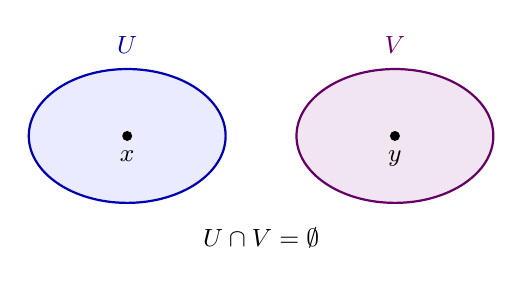
\begin{tikzpicture}[font=\small]
  \draw[blue!70!black, thick, fill=blue!8] (0,0) ellipse [x radius=1.25, y radius=0.85];
  \draw[violet!80!black, thick, fill=violet!10] (3.4,0) ellipse [x radius=1.25, y radius=0.85];
  \fill (0,0) circle (1.8pt) node[below=2pt] {$x$};
  \fill (3.4,0) circle (1.8pt) node[below=2pt] {$y$};
  \node[blue!70!black] at (0,1.15) {$U$};
  \node[violet!80!black] at (3.4,1.15) {$V$};
  \node at (1.7,-1.3) {$U \cap V = \emptyset$};
\end{tikzpicture}

  \caption{T2 (Hausdorff): farklı $x,y$ noktaları, kesişmeyen $U\ni x$
    ve $V\ni y$ açıklarıyla ayrılır.}
  \label{fig:ch06:t2}
\end{figure}

\begin{figure}[ht]
  \centering
  \begin{tikzpicture}[font=\small]
  \fill (0,0) circle (1.8pt) node[below=3pt] {$x$};
  \draw[blue!70!black, thick] (0,0.05) ellipse [x radius=1.0, y radius=0.72];
  \node[blue!70!black] at (0,1.05) {$U$};
  \draw[red!70!black, thick, fill=red!6, pattern=north east lines, pattern color=red!40]
    plot[smooth cycle, tension=0.9] coordinates
    {(3.3,-0.3) (4.4,-0.5) (5.0,0.4) (4.0,0.9) (3.2,0.5)};
  \node[red!70!black] at (4.15,-1.0) {$F$ (kapalı)};
  \draw[violet!80!black, thick] (4.1,0.15) ellipse [x radius=1.55, y radius=1.2];
  \node[violet!80!black] at (4.1,1.6) {$V$};
  \node at (2.05,-1.75) {$x\notin F,\qquad x\in U,\quad F\subseteq V,\quad U\cap V=\emptyset$};
\end{tikzpicture}

  \caption{Regülerlik: $x$ noktası ile onu içermeyen kapalı $F$ kümesi,
    ayrık $U$ ve $V$ açıklarına konabilir. T3 bunun üstüne T1 ister.}
  \label{fig:ch06:t3}
\end{figure}

\begin{karsiornek}
Hiçbir ayrılma aksiyomunu sağlamayan uzay: iki noktalı indirgenmiş
uzay. Açıklar yalnız $\emptyset$ ve $X$ olduğundan iki noktayı ayıran
\emph{hiçbir} açık yoktur --- uzay T0 bile değildir. Örnekler
bölümünde \texttt{two\_point\_indiscrete\_space()} ile test edilir;
zincirin en altının da boş kalabileceğini gösterir.
\end{karsiornek}

%% ============================================================
\section{Teoremler}
%% ============================================================

\begin{theorem}[Ayrılma Zinciri]
T4 $\Rightarrow$ T3.5 $\Rightarrow$ T3 $\Rightarrow$ T2.5 $\Rightarrow$ T2 $\Rightarrow$ T1
$\Rightarrow$ T0. Tersi genel olarak doğru değildir.
\end{theorem}

\begin{proof}[Rehberli Kanıt --- model halka: T2 $\Rightarrow$ T1]
$x\neq y$ verilsin. T2 ile ayrık $U\ni x$, $V\ni y$ açıkları vardır.
$U\cap V=\emptyset$ olduğundan $y\notin U$ ve $x\notin V$: hem
``$x$'i içerip $y$'yi dışlayan'' hem ``$y$'yi içerip $x$'i dışlayan''
açık bulundu --- T1'in iki yönlü koşulu sağlandı. Kalan halkalar
(T1 $\Rightarrow$ T0 dahil) aynı şablonla Alıştırma~T1'de
kanıtlanır.
\end{proof}

\begin{figure}[ht]
  \centering
  \begin{tikzpicture}[font=\small, node distance=9mm,
    aks/.style={draw, rounded corners, fill=blue!6, inner sep=5pt}]
  \node[aks] (t4) {T4};
  \node[aks, right=of t4] (t35) {T3.5};
  \node[aks, right=of t35] (t3) {T3};
  \node[aks, right=of t3] (t25) {T2.5};
  \node[aks, right=of t25] (t2) {T2};
  \node[aks, right=of t2] (t1) {T1};
  \node[aks, right=of t1] (t0) {T0};
  \foreach \a/\b in {t4/t35, t35/t3, t3/t25, t25/t2, t2/t1, t1/t0}
    \draw[-{Stealth[length=2.6mm]}, thick] (\a) -- (\b);
  \draw[red!70!black, -{Stealth[length=2.2mm]}, dashed]
    (t1.south) to[bend right=40] node[below=14pt, font=\scriptsize, align=center]
    {geçmez: kosonlu $\mathbb{N}$\\ (T1, T2 değil)} (t2.south);
  \draw[red!70!black, -{Stealth[length=2.2mm]}, dashed]
    (t0.south) to[bend right=40] node[below=35pt, font=\scriptsize, align=center]
    {geçmez: Sierpiński\\ (T0, T1 değil)} (t1.south);
\end{tikzpicture}

  \caption{Ayrılma zinciri: düz oklar implikasyonları gösterir.
    Kesikli kırmızı oklar terslerin \emph{geçmediği} iki kanonik
    karşı-örneği işaretler; her ikisi de bu kılavuzun örnekleridir
    (Örnek~1 ve Örnek~2).}
  \label{fig:ch06:zincir}
\end{figure}

\begin{theorem}[Urysohn Fonksiyon Teoremi]
$X$ normal ise ve $C, D$ disjoint kapalı kümeler ise, $f: X \to [0,1]$ sürekli vardır:
$f|_C \equiv 0$, $f|_D \equiv 1$.
\end{theorem}

\begin{proof}[İspat eskizi]
Normallikle $C \subseteq U_{1/2}$, $\overline{U_{1/2}} \cap D = \emptyset$
olan açık $U_{1/2}$ seç. Aynı adımı tekrarlayıp her ikili kesir
$q = k/2^n \in [0,1]$ için, $p < q \Rightarrow \overline{U_p} \subseteq U_q$
koşulunu sağlayan iç-içe açıklar ailesi $\{U_q\}$ kur (normallik her ekleme
adımını mümkün kılar). Sonra $f(x) = \inf\{q : x \in U_q\}$ (hiç içermiyorsa
$1$) tanımla; iç-içe geçme süreklilik verir, $C$ üzerinde $0$, $D$ üzerinde
$1$ alınır.
\end{proof}

\begin{figure}[ht]
  \centering
  \begin{tikzpicture}[font=\small]
  \draw[rounded corners=8pt, thick] (-0.4,-1.15) rectangle (6.4,1.45);
  \node at (5.95,1.2) {$X$};
  \draw[blue!70!black, thick, fill=blue!10] (0.8,0.15) ellipse [x radius=0.85, y radius=0.6];
  \node[blue!70!black] at (0.8,0.15) {$C$};
  \draw[red!70!black, thick, fill=red!10] (5.2,0.15) ellipse [x radius=0.85, y radius=0.6];
  \node[red!70!black] at (5.2,0.15) {$D$};
  \draw[-{Stealth}] (7.7,-0.9) -- (7.7,1.3);
  \draw (7.6,-0.6) -- (7.8,-0.6) node[right] {$0$};
  \draw (7.6,1.0) -- (7.8,1.0) node[right] {$1$};
  \draw[blue!70!black, -{Stealth}, dashed]
    (1.7,0.0) to[bend right=14] node[below, font=\scriptsize, pos=0.45] {$f$} (7.58,-0.6);
  \draw[red!70!black, -{Stealth}, dashed] (6.1,0.3) to[bend left=10] (7.58,1.0);
  \node[font=\scriptsize, align=center] at (3.0,-1.65)
    {$f$ sürekli; $f|_C\equiv 0$, $f|_D\equiv 1$; ara bölgede $0$ ile $1$ arası değerler};
\end{tikzpicture}

  \caption{Urysohn fonksiyonu: normal uzayda ayrık kapalı $C$ ve $D$
    için $f|_C\equiv 0$, $f|_D\equiv 1$ olan sürekli $f:X\to[0,1]$
    vardır; uzay, iki kapalı küme arasında ``sürekli geçiş'' yapacak
    kadar zengindir.}
  \label{fig:ch06:urysohn}
\end{figure}

\begin{nedenonemli}
Urysohn teoremi, küme dilindeki bir ayırma özelliğini (normallik)
\emph{sürekli fonksiyon üretimine} çevirir. Tietze Genişleme bunun
doğrudan sonucudur ve metrikleştirme teoremlerinin (Bölüm~9 sonrası
ufuk) temel aracıdır: fonksiyon üretebilen uzay, metrik benzeri
yapılar kurabilen uzaydır.
\end{nedenonemli}

\begin{theorem}[Tietze Genişleme]
$X$ normal ise her kapalı $A \subseteq X$ üzerinde $f: A \to [a,b]$ süreklisi
tüm $X$'e sürekli genişletilebilir.
\end{theorem}

\begin{theorem}[Tychonoff Karakterizasyonu]
$X$, T3.5'tir $\iff$ $X$ bir küp $[0,1]^I$'ya homeomorf gömülebilir.
\end{theorem}

\begin{proof}[İspat eskizi]
($\Leftarrow$) $[0,1]^I$ bir kompakt Hausdorff çarpımdır, dolayısıyla
T3.5'tir; T3.5 kalıtsaldır, alt-uzaya geçer. ($\Rightarrow$) $X$ tam regüler
ise $I = C(X,[0,1])$ (tüm sürekli $[0,1]$-değerli fonksiyonlar) indeks kümesini
al; değerlendirme gömmesi $e(x) = (f(x))_{f\in I}$ tanımla. Tam regülerlik,
$e$'nin birebir ve homeomorfik bir gömme olmasını sağlar --- her nokta--kapalı
çift bir $f$ ile ayrıldığından.
\end{proof}

\begin{theorem}[Sonlu T1 $\iff$ Ayrık]
Sonlu bir uzayda T1 $\iff$ ayrık topoloji.
\end{theorem}
\begin{proof}[Rehberli Kanıt]
\textbf{Strateji:} T1'den tekillerin kapalılığına, oradan sonlu
birleşimle her alt kümenin kapalılığına yürünür.
\begin{enumerate}
  \item ($\Rightarrow$) T1 gereği her $y\neq x$ için $y\in U_y$,
        $x\notin U_y$ olan açık $U_y$ vardır;
        $X\setminus\{x\}=\bigcup_{y\neq x}U_y$ açıktır, yani $\{x\}$
        kapalıdır.
  \item Herhangi $A\subseteq X$, \emph{sonlu} sayıda tekilin birleşimi
        olarak kapalıdır (kapalıların sonlu birleşimi kapalıdır).
  \item Her $A$ kapalı ise her $X\setminus A$ açıktır; $A$ keyfî
        olduğundan her alt küme açıktır: topoloji ayrıktır.
  \item ($\Leftarrow$) Ayrık topolojide her $\{x\}$ açıktır; $x\neq y$
        çifti $\{x\}$ ve $\{y\}$ ile iki yönlü ayrılır: T1 (hatta T2).
\end{enumerate}
Sonsuzlukta 2.~adım çöker: sonsuz birleşim kapalılığı korumaz ---
kosonlu $\mathbb{N}$ tam bu nedenle T1 olup ayrık değildir.
\end{proof}

\noindent Bu teorem, Bölüm~\ref{ch:topological_spaces} K1
alıştırmasındaki gözlemin --- üç noktalı kosonlu uzayın ayrık çıkması
--- genel açıklamasıdır.

\begin{theorem}[Kompakt $+$ Hausdorff $\Rightarrow$ T4]
Her kompakt Hausdorff uzay normaldir (T4).
\end{theorem}
\begin{proof}[İspat eskizi]
Önce ``kompakt Hausdorff $\Rightarrow$ regüler''i kur: $x \notin C$ (kapalı,
dolayısıyla kompakt) ise, her $c \in C$ için Hausdorff ayrık $U_c \ni x$,
$V_c \ni c$ verir; $\{V_c\}$ ailesi $C$'yi örter, kompaktlıkla sonlu alt-örtü
$V_{c_1},\dots,V_{c_n}$ al. $U = \bigcap_i U_{c_i}$ ve $V = \bigcup_i V_{c_i}$
aradığın ayrık açıkları verir. Sonra aynı argümanı bir nokta yerine ikinci bir
kapalı (kompakt) $D$ kümesine uygula: her $d \in D$ için regülerlik ayrık
$U_d \supseteq C$, $W_d \ni d$ verir; $D$ kompakt olduğundan sonlu alt-örtüyle
$C$ ve $D$ ayrık açıklara konur --- normallik tam budur.
\end{proof}

\noindent Bu, Kompaktlık bölümündeki ``kompakt $+$ Hausdorff
$\Rightarrow$ T4'' teoreminin ayrılma-aksiyomu tarafıdır; kompaktlık, sonsuz
Hausdorff ayrımlarını \emph{sonlu} sayıya indirgeyerek normalliği mümkün kılar.

%% ============================================================
\section{Algoritmalar}
%% ============================================================

\begin{algorithm}
\caption{Sonlu T0 Karar Prosedürü}
\begin{algorithmic}[1]
\For{each pair $(x, y)$ with $x \neq y$}
    \If{$\nexists U \in \tau$: $(x \in U \wedge y \notin U)$ or $(y \in U \wedge x \notin U)$}
        \Return \textbf{false}
    \EndIf
\EndFor
\Return \textbf{true}
\end{algorithmic}
\end{algorithm}

\noindent\textbf{Karmaşıklık T0:} $O(|X|^2 \cdot |\tau|)$. \quad
\textbf{Karmaşıklık T2:} $O(|X|^2 \cdot |\tau|^2)$.

\subsection{İz Sürme: T0 Prosedürü Sierpiński Üzerinde}

$X=\{0,1\}$, $\tau=\{\emptyset,\{1\},X\}$:

\begin{table}[ht]
\centering
\begin{tabular}{llccl}
\toprule
\textbf{Çift} $(x,y)$ & \textbf{Denenen} $U$ &
$x\in U \wedge y\notin U$ & $y\in U \wedge x\notin U$ & \textbf{Karar} \\
\midrule
$(0,1)$ & $\emptyset$ & hayır & hayır & devam \\
$(0,1)$ & $\{1\}$ & hayır & \textbf{evet} & çift ayrıldı \\
--- & --- & --- & --- & tüm çiftler bitti $\to$ \textbf{true} \\
\bottomrule
\end{tabular}
\caption{Tek çift tek açıkla ayrılır; genel sınır
  $O(|X|^2\cdot|\tau|)$'dur.}
\end{table}

%% ============================================================
\section{pytop API}
%% ============================================================

\begin{lstlisting}[language=Python, caption={Ayrılma aksiyom importları}]
from pytop import (
    is_t0, is_t1, is_t2, is_t2_5, is_t3, is_t4,
    is_hausdorff, is_regular, is_normal, is_perfectly_normal,
    separation_chain, analyze_separation,
)
\end{lstlisting}

\begin{table}[h]
\centering
\begin{tabular}{lll}
\toprule
\textbf{Fonksiyon} & \textbf{İmza} & \textbf{Açıklama} \\
\midrule
\texttt{is\_t0} \ldots \texttt{is\_t4} & \texttt{(space)} & Aksiyom kontrolü \\
\texttt{separation\_chain} & \texttt{(space)} & Tüm zincir: \texttt{dict[str, Result]} \\
\texttt{analyze\_separation} & \texttt{(space, property='hausdorff')} & Tek aksiyom sorgu \\
\bottomrule
\end{tabular}
\caption{Ayrılma fonksiyonları}
\end{table}

\begin{nedenonemli}
\texttt{is\_*} yüklemleri ham \texttt{bool} değil, \texttt{.status}
alanı \texttt{true} / \texttt{false} / \texttt{unknown} olabilen bir
\texttt{Result} döndürür. Üçüncü değer dürüstlüktür: örneğin T3.5
(Tychonoff) sürekli fonksiyonlarla tanımlanır ve sonlu açık-küme
taramasıyla karar verilemez; \texttt{separation\_chain} bu durumda
\texttt{tychonoff: unknown} raporlar. Sembolik uzaylarda da
bilinmeyen özellikler \texttt{unknown} kalır --- kütüphane bilmediğini
\emph{bilmediğini söyleyerek} belirtir.
\end{nedenonemli}

%% ============================================================
\section{Örnekler}
%% ============================================================

\subsection{Örnek 1: Sierpiński — T0 $\checkmark$, T1 $\times$}

\begin{lstlisting}[language=Python]
from pytop import sierpinski_space, is_t0, is_t1, is_t2
s = sierpinski_space()
print("T0:", is_t0(s).status)
print("T1:", is_t1(s).status)
print("T2:", is_t2(s).status)
\end{lstlisting}
\begin{lstlisting}[caption={Çıktı}]
T0: true
T1: false
T2: false
\end{lstlisting}

\paragraph{Ne oldu?}
\texttt{T0: true} --- $(0,1)$ çifti için $\{1\}$ açığı $1$'i içerir,
$0$'ı dışlar; tek çift bu olduğundan T0 tamam. \texttt{T1: false} ---
ters yön yok: $0$'ı içerip $1$'i dışlayan açık küme yoktur
($\{0\}\notin\tau$; bkz.\ Bölüm~\ref{ch:topological_spaces},
Örnek~1). T1 düşünce T2 de düşer. Sierpiński, zincirin ``T0'da
takılan'' kanonik örneğidir (Şekil~\ref{fig:ch06:zincir}).

\subsection{Örnek 2: Kosonlu $\mathbb{N}$ — T1 $\checkmark$, T2 $\times$}

\begin{lstlisting}[language=Python]
from pytop import naturals_cofinite, is_t1, is_t2
nc = naturals_cofinite()
print("T1:", is_t1(nc).status)
print("T2:", is_t2(nc).status)
\end{lstlisting}
\begin{lstlisting}[caption={Çıktı}]
T1: true
T2: false
\end{lstlisting}

\paragraph{Ne oldu?}
\texttt{T1: true} --- her $n$ için $\mathbb{N}\setminus\{n\}$
kosonludur, dolayısıyla açıktır; bu, her noktayı diğerinden iki yönlü
ayırır. \texttt{T2: false} --- boş olmayan iki kosonlu açık $U,V$
daima kesişir: $\mathbb{N}\setminus(U\cap V)=
(\mathbb{N}\setminus U)\cup(\mathbb{N}\setminus V)$ iki sonlu kümenin
birleşimi olarak sonludur; $\mathbb{N}$ sonsuz olduğundan
$U\cap V\neq\emptyset$. Bu örnek,
Bölüm~\ref{ch:topological_spaces}~K1'in ``neden sonsuz taşıyıcı
gerekir'' sorusunun cevabıdır.

\subsection{Örnek 3: Ayrılma Zinciri — Ayrık}

\begin{lstlisting}[language=Python]
from pytop import discrete_topology, separation_chain
d = discrete_topology(1, 2, 3)
for prop, result in separation_chain(d).items():
    print(f"  {prop:20s}: {result.status}")
\end{lstlisting}
\begin{lstlisting}[style=output, caption={Çıktı}]
  t0                  : true
  t1                  : true
  hausdorff           : true
  urysohn             : true
  t3                  : true
  tychonoff           : true
  t4                  : true
  completely_normal   : true
  perfectly_normal    : true
\end{lstlisting}

\paragraph{Ne oldu?}
Ayrık uzayda her tekil açık olduğundan her ayırma görevi tekil
komşuluklarla çözülür; dokuz yüklemin tümü \texttt{true} döner.
\texttt{tychonoff} bile \texttt{true}'dur: ayrık uzayda her fonksiyon
süreklidir, ayırıcı fonksiyon doğrudan yazılır.
\texttt{separation\_chain}'in anahtar sırası zincirin mantıksal
sırasıdır --- bir uzayın ``nerede takıldığını'' yukarıdan aşağı
okuyabilirsiniz (krş.\ Alıştırma~K2).

\subsection{Örnek 4: Regüler Ama T3 Değil --- Konvansiyon Testi}

\begin{lstlisting}[language=Python]
from pytop import two_point_indiscrete_space, is_regular, is_normal, is_t3, is_t4

tp = two_point_indiscrete_space()
print("regular:", is_regular(tp).status, "| normal:", is_normal(tp).status)
print("t3     :", is_t3(tp).status, "| t4    :", is_t4(tp).status)
\end{lstlisting}

\begin{lstlisting}[style=output, caption={Çıktı}]
regular: true | normal: true
t3     : false | t4    : false
\end{lstlisting}

\paragraph{Ne oldu?}
İndirgenmiş iki noktalı uzayda kapalı kümeler yalnız $\emptyset$ ve
$X$'tir; ``nokta--kapalı'' ve ``kapalı--kapalı'' ayırma koşullarının
öncülü hiç gerçekleşmez, koşullar boş yere sağlanır:
\texttt{regular} ve \texttt{normal} \texttt{true}. Ama uzay T1
olmadığından (tekiller kapalı değil) \texttt{t3} ve \texttt{t4}
\texttt{false} kalır --- ``Dikkat'' kutusundaki konvansiyonun
davranışsal kanıtı.

\subsection{Örnek 5: Dışlanan-Nokta Topolojisi --- İkinci Bir ``T0'da Takılan''}

Sierpiński, T0-olup-T1-olmayan tek örnek değildir. $X=\{0,1,2\}$ üzerinde
\textbf{dışlanan-nokta topolojisi} ($0$ dışlanır): bir küme ya $0$'ı içermez ya
da $X$'in kendisidir.

\begin{lstlisting}[language=Python]
from pytop import excluded_point_topology, is_t0, is_t1, separation_chain

ep = excluded_point_topology(3, 0)   # X = {0,1,2}, dislanan nokta 0
print("T0:", is_t0(ep).status, "| T1:", is_t1(ep).status)
for prop, result in separation_chain(ep).items():
    print(f"  {prop:20s}: {result.status}")
\end{lstlisting}
\begin{lstlisting}[style=output, caption={Çıktı}]
T0: true | T1: false
  t0                  : true
  t1                  : false
  hausdorff           : false
  urysohn             : false
  t3                  : false
  tychonoff           : false
  t4                  : false
  completely_normal   : false
  perfectly_normal    : false
\end{lstlisting}

\paragraph{Ne oldu?}
\texttt{T0: true} --- $1$ ve $2$, $0$-içermeyen $\{1\}$/$\{2\}$ açıklarıyla iki
yönlü ayrılır; $0$ ile herhangi bir nokta arasında ise $0$'ı dışlayan açık tek
yönlü ayrım verir. \texttt{T1: false} --- $0$'ı içeren tek açık $X$'tir,
dolayısıyla $\{0\}$ kapalı değildir. Sierpiński'den farklı bir mekanizmayla
zincir yine T0'da takılır.

\subsection{Örnek 6: Metrik Uzaylar --- Zincirin Tepesine Kadar}

Her metrik uzay normaldir (T4) ve zincirin tüm üst basamaklarını sağlar; bunu
$\mathbb{R}$ ve $[0,1]$ üzerinde gözlemleyelim.

\begin{lstlisting}[language=Python]
from pytop import real_line_metric, closed_unit_interval_metric
from pytop import is_t2, is_urysohn, is_t3, is_t4

rl = real_line_metric()
ui = closed_unit_interval_metric()
print("R         t2/urysohn/t3/t4:", is_t2(rl).status, is_urysohn(rl).status, is_t3(rl).status, is_t4(rl).status)
print("[0,1]     t2/urysohn/t3/t4:", is_t2(ui).status, is_urysohn(ui).status, is_t3(ui).status, is_t4(ui).status)
\end{lstlisting}
\begin{lstlisting}[style=output, caption={Çıktı}]
R         t2/urysohn/t3/t4: true true true true
[0,1]     t2/urysohn/t3/t4: true true true true
\end{lstlisting}

\paragraph{Ne oldu?}
Metrik mesafe kendisi bir ayırıcıdır: ayrık kapalı $C, D$ için
$f(x) = d(x,C)/(d(x,C)+d(x,D))$ sürekli Urysohn fonksiyonunu doğrudan verir ---
yani metrik uzaylar yalnız T2 değil, T4'e kadar her aksiyomu sağlar
(Teorem~2.2'nin metrik durumda elle yazılabilen tanığı). Ayrılma zincirinin
sonlu/sembolik örneklerle metrik örnekler arasındaki keskin farkı budur.

%% ============================================================
\section{Alıştırmalar}
%% ============================================================

\subsection*{Kodlama}
\begin{enumerate}[label=\textbf{K\arabic*.}]
  \item \label{ex:ch06:K1} \texttt{make\_topology(\{1,2,3\},\{1\},\{2\},\{1,2\})}
        için \texttt{separation\_chain} çalıştırın; her sonucu yorumlayın.
        \ipucu{Önce açıkları listeleyin:
        $\emptyset,\{1\},\{2\},\{1,2\},X$. Her çifti ayıran açık
        arayın; $3$'ü içerip $1$'i dışlayan açık var mı?}
        (\hyperref[sol:ch06:K1]{çözüm})

  \item \label{ex:ch06:K2} \texttt{finite\_chain\_space(3)} üzerinde en
        yüksek sağlanan aksiyomu bulun.
        \ipucu{Çıktıda \texttt{true} olan en güçlü anahtarı arayın;
        \texttt{unknown} değerlerini ``Neden önemli?'' kutusuna göre
        yorumlayın.}
        (\hyperref[sol:ch06:K2]{çözüm})

  \item \label{ex:ch06:K3} \texttt{two\_point\_indiscrete\_space()}
        üzerinde T0, T1, T2 test edin.
        \ipucu{Tek boş olmayan açık $X$ iken herhangi bir çift nasıl
        ayrılabilir?}
        (\hyperref[sol:ch06:K3]{çözüm})

  \item \label{ex:ch06:K4} \texttt{excluded\_point\_topology(4, 0)} (yani
        $X=\{0,1,2,3\}$, dışlanan nokta $0$) üzerinde
        \texttt{separation\_chain} çalıştırın; sağlanan en yüksek aksiyomu
        belirleyin ve neden T1'in düştüğünü açıklayın.
        \ipucu{$0$'ı içeren tek açık $X$'tir; $\{0\}$ kapalı mı?}
        (\hyperref[sol:ch06:K4]{çözüm})
\end{enumerate}

\subsection*{Teori}
\begin{enumerate}[label=\textbf{T\arabic*.}]
  \item \label{ex:ch06:T1} T2 $\Rightarrow$ T1 $\Rightarrow$ T0
        implikasyonlarını kanıtlayın.
        \ipucu{T2 $\Rightarrow$ T1: ayrık $U\ni x$, $V\ni y$
        verildiğinde $U$, $y$'yi; $V$, $x$'i dışlar --- iki yönlü ayrım
        hazır. T1 $\Rightarrow$ T0: iki yönlü ayrım tek yönlüyü içerir.}
        (\hyperref[sol:ch06:T1]{çözüm})

  \item \label{ex:ch06:T2} Sonlu uzayda T1 $\iff$ ayrık topoloji
        olduğunu gösterin.
        \ipucu{T1 $\Rightarrow$ tekiller kapalı $\Rightarrow$ (sonlu
        birleşim) her alt küme kapalı $\Rightarrow$ her alt küme açık.}
        (\hyperref[sol:ch06:T2]{çözüm})

  \item \label{ex:ch06:T3} Her metrik uzayın normal (T4) olduğunu
        kanıtlayın.
        \ipucu{Ayrık kapalı $C, D$ için
        $f(x) = d(x,C)/(d(x,C)+d(x,D))$ sürekli Urysohn fonksiyonunu yazın;
        $f^{-1}([0,\tfrac12))$ ve $f^{-1}((\tfrac12,1])$ aradığınız ayrık
        açıklardır.}
        (\hyperref[sol:ch06:T3]{çözüm})
\end{enumerate}
